% Ignore 'User Regex' warnings:
% chktex-file 44 


\documentclass[12pt]{article}

\usepackage{graphicx,url}
\usepackage{caption}
\usepackage{subcaption}
\usepackage{wrapfig}

\usepackage[british]{babel}
\usepackage[utf8]{inputenc}  

\begin{document} 

\section{Volatility Calculation}

The purpose of this report was to estimate the volatility historical stock prices based on four sample datasets spanning a 170 day period. The data included biases and errors which required cleaning and the resulting code was designed to run automatically and unsupervised as part of a scheduled set of tasks.

\begin{figure}[ht]
  \centering
  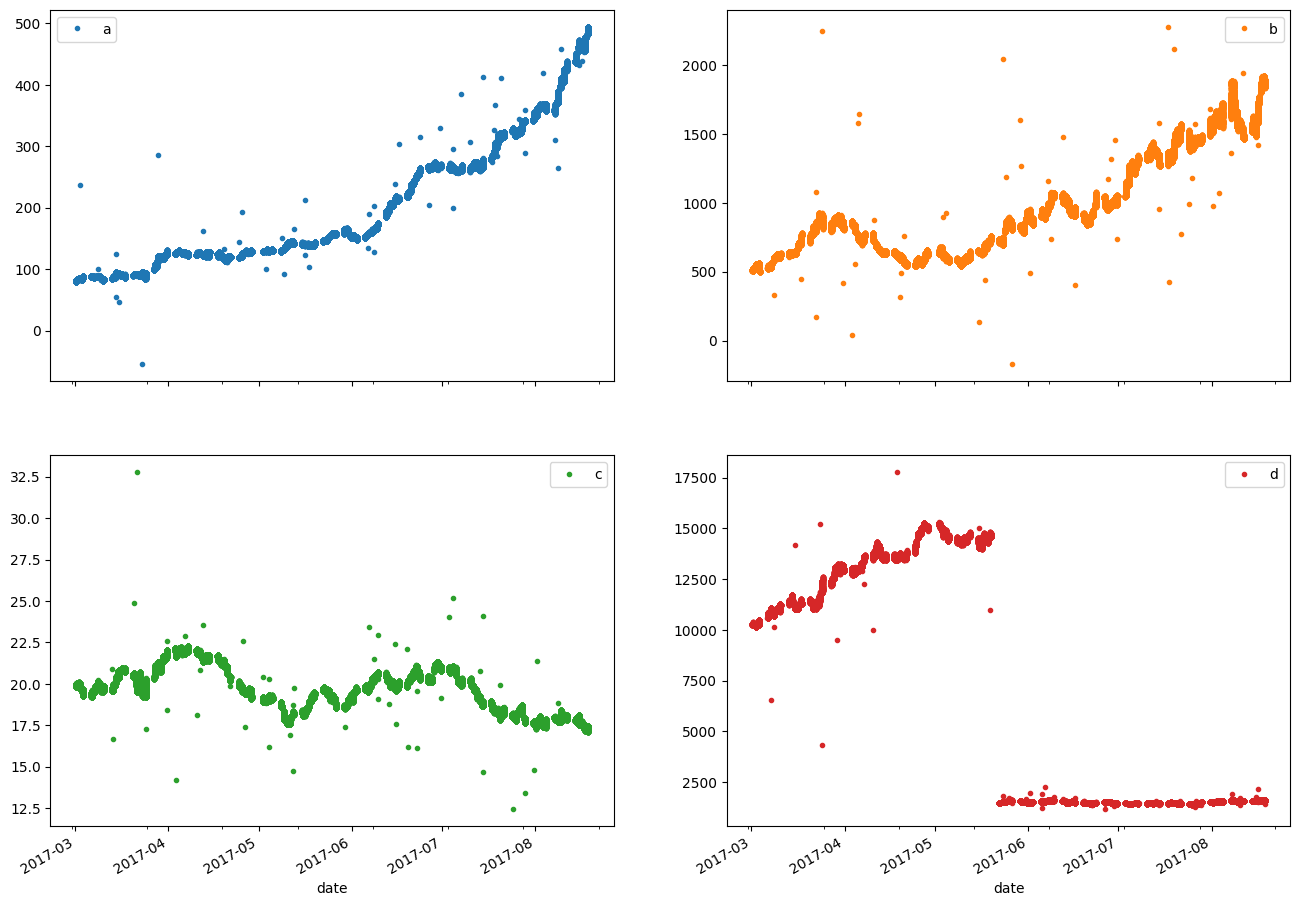
\includegraphics[width=\textwidth]{raw-data.png}
  \caption{Raw data for four stock trade time series.}\label{fig:rawdata}
\end{figure}

% Key observations from the raw data:

% \begin{itemize}
%     \item There are clear periodic gaps, signifying weekends in which no trading can occur.
%     \item Outliers clearly exist. The negative values seen in stocks a and b show that at least a number of these must be errors in data entry.
%     \item there is a significant change in behaviour at the mid point for stock d, which requires further handling.
%     \item Stock c appears to show increasing levels of volatility over time. Whether this is significant is dependent upon domain requirements and is explored later.
% \end{itemize}


\section{Outlier Detection}

We are interested primarily in \textit{additive outliers} which are defined as a type of outlier which does not affect the trend within the data and typically caused by data entry or human error. 

We use the two-sided median method of outlier detection: for a given point in time, $y_t$, the median value $m_t^{(k)}$ is computed within a $2k$ neighbourhood of point $y_t$. Where the absolute difference between $y_t$ and the median exceeds a threshold $\tau$, $y_t$ is identified as an outlier.\cite{basu2007automatic, pearson2002data} 

% Outlier detection is an ongoing area of research and the methods used in this report were constrained by the time allotted. Further work developing and validating these approaches for real-world implementation is warranted.

\begin{figure}[ht]
\centering
\begin{subfigure}{.5\textwidth}
  \centering
  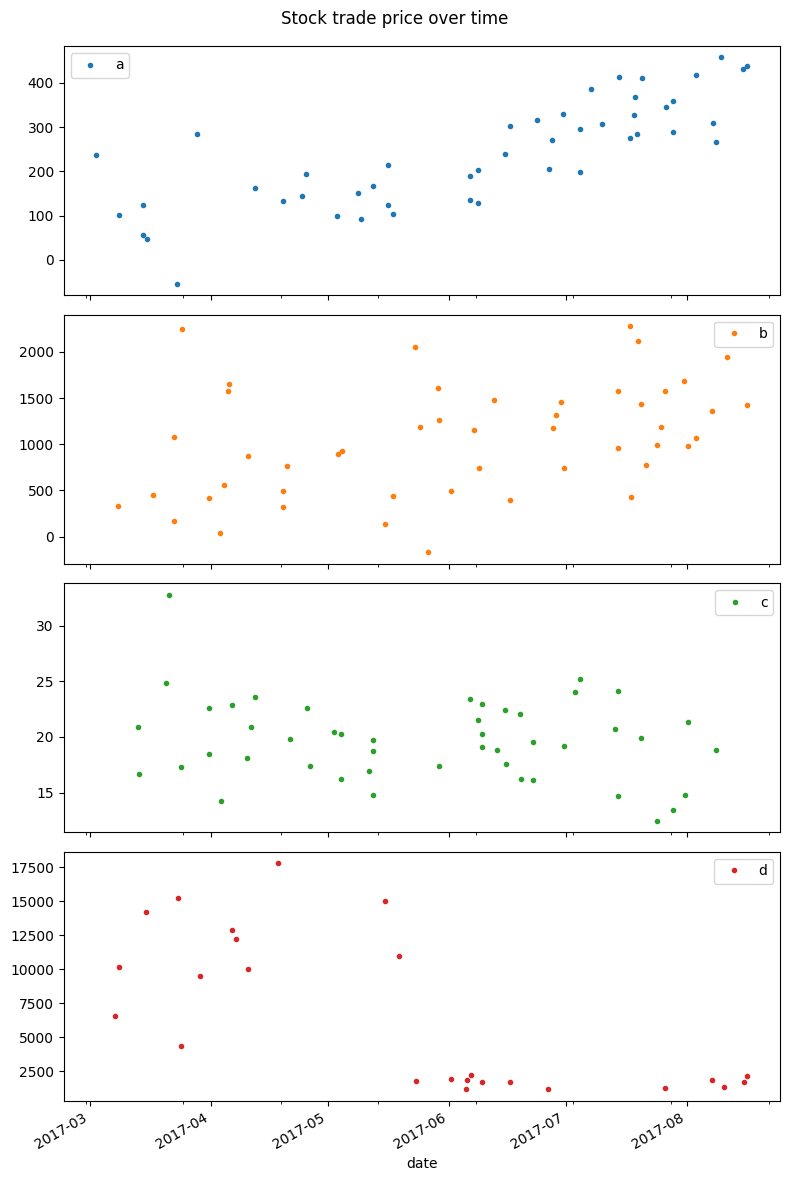
\includegraphics[width=\linewidth]{outliers.png}
  \caption{Outliers detected in data.}
\end{subfigure}%
\begin{subfigure}{.5\textwidth}
  \centering
  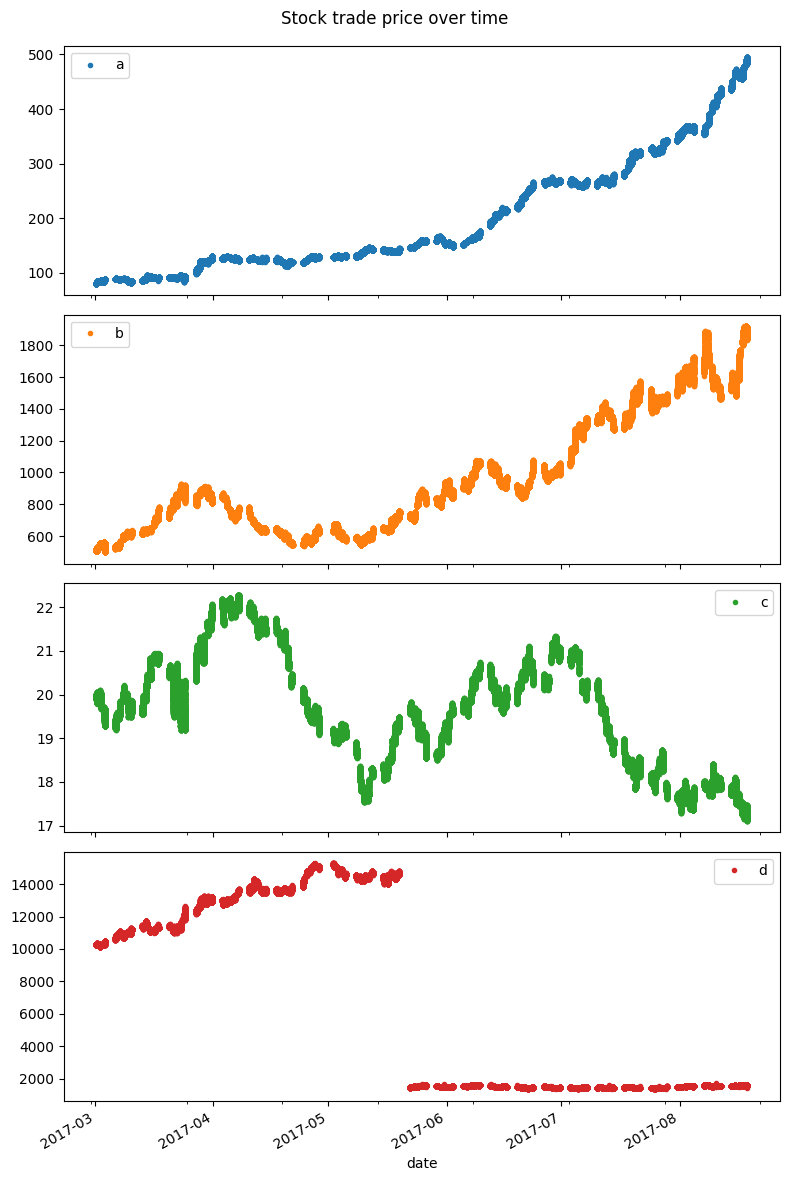
\includegraphics[width=\linewidth]{cleaned-data.png}
  \caption{Cleaned data.}
\end{subfigure}
\caption{Outlier detection and removal.}\label{fig:outliers}
\end{figure}


\section{Volatility Calculation}
The volatility calculation was based on the percentage annualised volatility of returns, given by the formula: $volatility = std \times \sqrt{252}$ where $std$ is the standard deviation of the daily rate of return. A key consideration for further work is to evaluate changes in volatility over time, as more recent trends may be more relevant to the application. Such changes are seen in the volatility plot for stock d (figure~\ref{fig:vol}), which becomes more volatile after the mid point of the series. Note that the outlier here represents the level shift and can be ignored for the purposes of this comparison.


\begin{figure}[ht]
\centering
\begin{subfigure}{.5\textwidth}
  \centering
  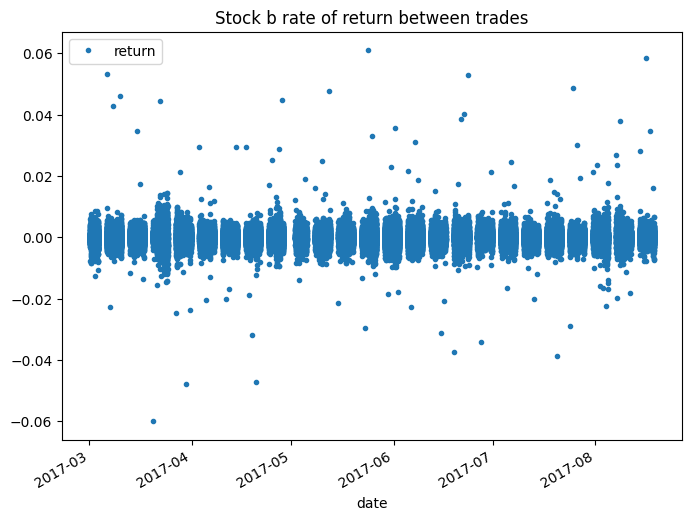
\includegraphics[width=\linewidth]{return-b.png}
  \caption{No change in volatility over time.}
\end{subfigure}%
\begin{subfigure}{.5\textwidth}
  \centering
  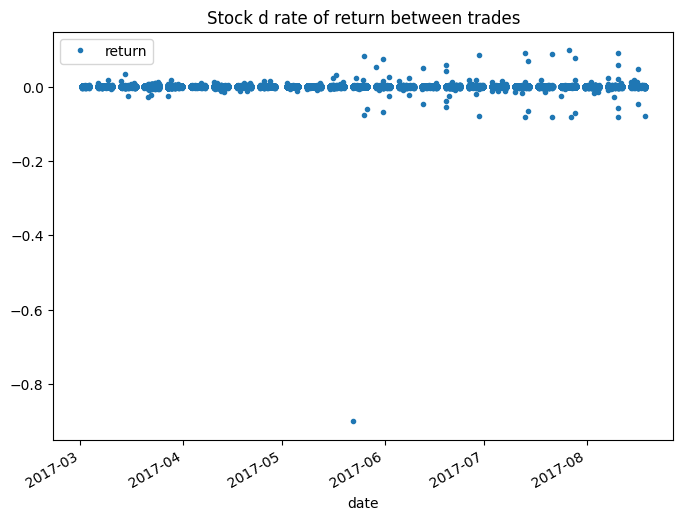
\includegraphics[width=\linewidth]{return-d.png}
  \caption{Increased volatility after mid point.}
\end{subfigure}
\caption{Comparison of volatility over time.}\label{fig:vol}
\end{figure}


Volatility is then calculated using the latest observed price for each day as an estimation of the closing price of each stock (table~\ref{tab:vol}).

\begin{table}[ht]
    \centering
    \begin{tabular}{|c|c|}
        \hline
        Stock & Volatility \\
        \hline
        A & 145.9\% \\
        B & 221.1\% \\
        C & 31.61\% \\
        D & 149.3\% \\
        \hline
    \end{tabular}
    \caption{Percentage annualised volatility.}\label{tab:vol}
\end{table}

\section{Further work}
If this process is to be performed every day (and small gains in efficiency are relevant), outlier detection can be performed once per time window and stored to the source data files rather than recalculating each day. It also assumes that data will be supplied in a relatively similar format --- further conformity checks are recommended. Finally, the level shift change exhibited in stock d is not handled as doing so was not within the specified requirements, not are changes in volatility over time, but the significance of this change should be discussed with domain experts.


\bibliographystyle{acm}
\bibliography{bib}


\end{document}
